% =========================
% 5_design.tex  --- calibrated tokenizer + label-free Phase A + evidence engine
% =========================
\section{Design of HALO}
\label{sec:design}

\subsection{System Overview}
\label{sec:overview}
\label{sec:requirements}

HALO is organised as two phases with a hard boundary (Figure~\ref{fig:overview}).
\textbf{Phase~A} learns a representation using no activity labels whatsoever; \textbf{Phase~B}
turns that frozen representation into a recogniser for whatever label set a deployment declares,
using labels only as annotations on stored exemplars. The boundary is where the argument of
Section~\ref{sec:motivation} lands: L1 says compatibility must be structural, so it belongs in
the encoder before any label is involved; L2 says the label decision must not be a projection
into text space, so it belongs after the encoder, in a component swappable per deployment.

\begin{figure*}[t]
    \centering
    \setlength{\abovecaptionskip}{4pt}
    \setlength{\belowcaptionskip}{-6pt}
  % PLACEHOLDER --- the system-overview figure is STALE and has been withdrawn from the manuscript.
%
% Why: the previous drawing labelled the encoder "two resolutions" and the loss box
% "masked latent + descriptor prediction". Both describe the pinned v2 artifact. The current
% repository default is a single fixed 1.0 s patch grid (multiresolution=False) with the
% descriptor term disabled (descriptor_weight=0), so the drawing no longer depicts the system.
%
% The previous TikZ source is preserved verbatim in figures/fig_overview_v2artifact.tex.
% Redraw from it once the checkpoint repin is decided. See STALENESS.md sec. 0 and sec. 2.
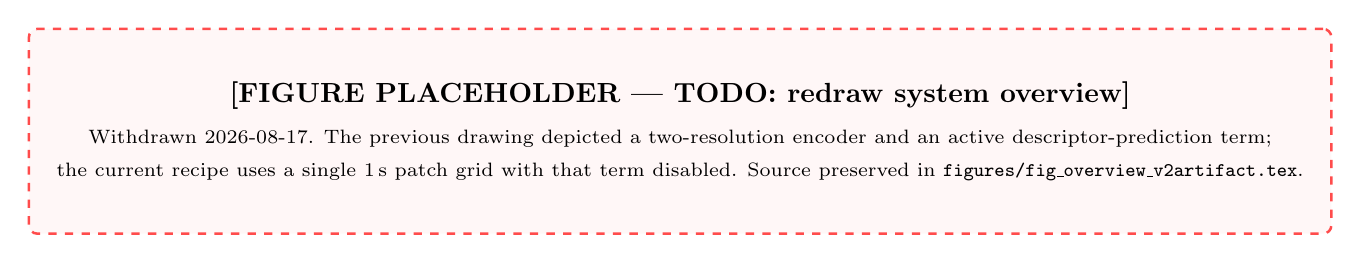
\begin{tikzpicture}
\node[draw=red!70,line width=0.9pt,dashed,rounded corners=3pt,inner sep=10pt,
      minimum width=0.96\textwidth,minimum height=26mm,align=center,fill=red!3]
  {\TODO{\textbf{[FIGURE PLACEHOLDER --- TODO: redraw system overview]}}\\[3pt]
   \scriptsize Withdrawn 2026-08-17. The previous drawing depicted a two-resolution encoder and an
   active descriptor-prediction term;\\
   \scriptsize the current recipe uses a single 1\,s patch grid with that term disabled.
   Source preserved in \texttt{figures/fig\_overview\_v2artifact.tex}.};
\end{tikzpicture}

  \caption{\textbf{HALO end to end.} One left-to-right path. Phase~A trains the tokenizer and
  encoder with objectives that never see an activity label. The encoder is then frozen and
  crosses the boundary unchanged---it is the \emph{same} weights that encode a query and that
  encoded every exemplar in memory, which is what lets the two be compared as vectors. Phase~B
  adds no parameters to that path: it appends encoded exemplars to a memory and accumulates
  evidence for the label strings declared at run time. Adding an activity, a placement, or a
  device is an append; no gradient step occurs anywhere to the right of \textsf{freeze}.}
  \label{fig:overview}
\end{figure*}

\textbf{One window, end to end.} A deployment hands HALO a $6$\,s window from whatever sensors it
has---say a $50$\,Hz watch accelerometer and gyroscope, six channels---plus one description string
per sensor and its list of activity names. The tokenizer cuts each channel into patches and turns
each patch into one token: a $32$-band constant-$Q$ readout on a frequency axis fixed in Hz, a
signed DC term carrying gravity, and two masks recording which of the $32$ bands this rate and
patch length could actually resolve. Nothing is resampled, so band $k$ denotes the same physical
frequency whether the device ran at $20$ or $100$\,Hz. Each token is then biased by the sentence
embedding of its sensor's description, and the token set---unordered over channels, positioned in
physical time---enters a $7.17$M-parameter transformer that emits one vector per patch. Those
vectors are the interface between the phases: Phase~A shapes them with objectives that never see
a label, and Phase~B compares them, by cosine similarity in that same space, against a memory of
encoded exemplars, accumulating evidence for whichever activity names were declared. The
demands of Section~\ref{sec:why} map onto this path one-to-one, and
Table~\ref{tab:mechanisms} fixes the name we use for each mechanism throughout. The distinctions
those names carry are the contribution: not ``a spectral tokenizer'' but one anchored to
\emph{physical} Hz; not a Nyquist mask but one bounded by the \emph{acquisition} clock; not
per-channel text but per-\emph{sensor}; not retrieval in CLIP space but in \emph{sensor} space.

\begin{table}[t]
  \centering
  \caption{Each deployment demand, the mechanism that answers it, and the name used for that
  mechanism throughout this paper. The qualifiers are load-bearing: each marks where HALO departs
  from the nearest existing technique. Rows 1--3 are the tokenizer
  (Section~\ref{sec:tokenizer_design}) and are what let one weight set accept any rate, channel
  count, and placement with no architectural change; rows 4--5 are the evidence engine
  (Section~\ref{sec:evidence_design}). Row 3 states a property we \emph{probe} rather than assert
  (Table~\ref{tab:tokenizer_ablation}), and row 5 is why no label budget requires a gradient
  update.}
  \label{tab:mechanisms}
  \scriptsize
  \setlength{\tabcolsep}{3pt}
  \begin{tabular}{@{}p{0.30\columnwidth} p{0.38\columnwidth} p{0.24\columnwidth}@{}}
    \toprule
    Demand & Mechanism & Name \\
    \midrule
    Rate and anti-aliasing differ per device
      & constant-$Q$ filterbank on a fixed physical-frequency axis over a native-rate transform;
        no resampling anywhere in the path
      & \textbf{physical-Hz tokenizer} \\[2pt]
    What a device \emph{could} measure differs
      & per-token masks bounded by the \textsc{acquisition} clock, not the rate the grid happens
        to be stored at
      & \textbf{acquisition-bounded observability masks} \\[2pt]
    Channel count, order and placement differ
      & free-text identity attached to the \textsc{sensor}, leaving channel count and order free
        while staying too coarse to fingerprint a corpus
      & \textbf{per-sensor language conditioning} \\[2pt]
    The label set belongs to the deployment
      & retrieve encoded exemplars by \textsc{sensor} similarity; accumulate evidence for whatever
        strings are declared at run time
      & \textbf{evidence retrieval in sensor space} \\[2pt]
    The label budget is small and fixed
      & append exemplars to memory; no gradient update at any budget
      & \textbf{append-only memory} \\
    \bottomrule
  \end{tabular}
\end{table}

\subsection{The Physical-Hz Tokenizer}
\label{sec:tokenizer_design}

\subsubsection{Per-sensor language conditioning: sensors, not channels}
\label{sec:sensor_grouping}

HALO's first commitment is that the unit of description is the \emph{sensor}, not the scalar
channel. Three co-located accelerometer axes share a coordinate frame: they rotate together,
experience the same gravity vector, and no physically realisable transformation moves one without
the others. Treating them as independent series discards this and lets per-channel text act as a
corpus fingerprint. HALO therefore models a stream as a \emph{set of sensors}, each a triad with
its own device, placement, and gravity convention---which also makes the augmentation physics
correct, since an $SO(3)$ rotation is applied jointly to a triad and its co-located gyroscope
rather than to a single axis.

Accelerometer streams are gravity-aware. The quasi-static component below the analysis band is
split off as a \emph{signed} per-axis DC feature rather than removed, so posture survives. On
$200$ real waist-phone windows each of standing, sitting and lying, the frequency path separates
no pair distinctly (all pairwise cosines within $0.84$--$0.88$) while signed DC places lying
nearly orthogonal to standing ($-0.04$); a design achieving orientation robustness through
\emph{invariance} discards that quantity, and with it the distinction between lying down
and standing still. Figure~\ref{fig:gravity} shows this and its
limit---standing and sitting stay at $0.99$ in DC, the same pair Section~\ref{sec:geometry} finds
inseparable in text, so neither path suffices alone. Because gravity conventions differ across
platforms, the convention is declared in the sensor's text and a gravity-removal augmentation is
applied with low probability, so the encoder sees both conventions for the same motion.

\subsubsection{A physical-frequency constant-$Q$ filterbank}
\label{sec:filterbank}

Each patch of each channel becomes one token entirely in the physical-frequency domain
(Appendix~\ref{app:tokenizer}, Figure~\ref{fig:tokenizer}). The patch is Hann-windowed and its DC
component removed, then
transformed by a zero-padded real DFT of fixed length $S{=}256$. The zero-padding is what makes
this rate-agnostic: for a patch sampled at rate $r$, DFT bin $m$ corresponds to physical frequency
$\phi[m] = mr/S$, so the \emph{same} matrix of bin indices maps to different Hz grids at different
rates, and the readout can be defined once in Hz. That readout is a constant-$Q$ Gaussian
filterbank~\cite{constantq,constantqfast} with $K{=}32$ centres log-spaced over $[0.3,15]$\,Hz at
$Q{=}4$. The limits are physical rather than tuned: gait cadence occupies $0.5$--$3$\,Hz, limb and
hand motion add harmonics to roughly $10$--$12$\,Hz, and content below $0.3$\,Hz is gravity, which
the signed DC feature already carries.

Rate-invariance is therefore a property of the construction rather than of a learned
approximation: a $2$\,Hz gait rhythm deposits energy in the same band whether the device sampled
at $20$ or $100$\,Hz, and because no interpolation exists in the path there is no aliasing to
introduce and no fabricated sample to explain away (Figure~\ref{fig:rateinv}). This is the
property, argued in Section~\ref{sec:no_grammar}, that rate-\emph{equivariance}~\cite{flowstate}
does not provide and that one flat cross-device memory requires.
Appendix~\ref{app:tokenizer} records the DFT- and patch-length guardrails.

\begin{figure*}[t]
    \centering
    \setlength{\abovecaptionskip}{4pt}
    \setlength{\belowcaptionskip}{-4pt}
  % =====================================================================
% fig_rateinvariance.tex --- L1 demonstrated on real data, not asserted.
%
% PROVENANCE: one 1.5 s accelerometer patch (x-axis) of `walking` from the
% NFI-FARED wrist stream, native 100 Hz, taken straight from the materialised
% native grid.  It is anti-alias resampled to 50 and 20 Hz with the same
% scipy.signal.resample_poly the data pipeline uses, then each version is run
% through the REAL PhysicalFilterbankTokenizer DSP path at ITS OWN rate
% (_spectral_power -> _apply_filterbank -> _observability_masks), exactly as in
% training.  Numbers generated 2026-07-26; cosines quoted in the caption are
% measured, not estimated.
% =====================================================================
\begin{tikzpicture}

% ---------------- LEFT: the same motion, three different arrays -------------
\begin{axis}[
  name=sigax,
  width=0.44\textwidth, height=3.5cm,
  xmin=0, xmax=1.5, ymin=-1.77, ymax=-0.18,
  xlabel={time (s)}, ylabel={accel. $x$ (g)},
  xlabel style={font=\scriptsize,yshift=2pt}, ylabel style={font=\scriptsize,yshift=-6pt},
  xticklabel style={font=\scriptsize}, yticklabel style={font=\scriptsize},
  axis line style={draw=halogray!60}, tick style={draw=halogray!60},
  title={\scriptsize\bfseries one 1.5\,s window, sampled three ways},
  title style={yshift=-2pt},
  scale only axis,
]
\addplot[draw=haloblue,line width=0.7pt] coordinates {(0.0000,-1.1792) (0.0100,-1.1394) (0.0200,-1.1194) (0.0300,-1.0986) (0.0400,-1.0708) (0.0500,-1.0366) (0.0600,-1.0066) (0.0700,-0.9902) (0.0800,-0.9707) (0.0900,-0.9561) (0.1000,-0.9524) (0.1100,-0.9502) (0.1200,-0.9458) (0.1300,-0.9424) (0.1400,-0.9404) (0.1500,-0.9377) (0.1600,-0.9299) (0.1700,-0.9158) (0.1800,-0.8989) (0.1900,-0.8796) (0.2000,-0.8623) (0.2100,-0.8489) (0.2200,-0.8398) (0.2300,-0.8318) (0.2400,-0.8323) (0.2500,-0.8416) (0.2600,-0.8640) (0.2700,-0.8933) (0.2800,-0.9204) (0.2900,-0.9470) (0.3000,-0.9734) (0.3100,-1.0027) (0.3200,-1.0342) (0.3300,-1.0784) (0.3400,-1.1106) (0.3500,-1.1260) (0.3600,-1.1213) (0.3700,-1.1206) (0.3800,-1.1357) (0.3900,-1.1826) (0.4000,-1.2510) (0.4100,-1.3142) (0.4200,-1.3569) (0.4300,-1.3755) (0.4400,-1.3899) (0.4500,-1.3965) (0.4600,-1.3850) (0.4700,-1.3582) (0.4800,-1.3274) (0.4900,-1.3040) (0.5000,-1.2817) (0.5100,-1.2454) (0.5200,-1.1995) (0.5300,-1.1467) (0.5400,-1.0938) (0.5500,-1.0571) (0.5600,-1.0432) (0.5700,-1.0430) (0.5800,-1.0503) (0.5900,-1.0557) (0.6000,-1.0542) (0.6100,-1.0457) (0.6200,-1.0251) (0.6300,-0.9944) (0.6400,-0.9580) (0.6500,-0.9282) (0.6600,-0.9070) (0.6700,-0.9019) (0.6800,-0.8979) (0.6900,-0.8923) (0.7000,-0.8909) (0.7100,-0.8772) (0.7200,-0.8604) (0.7300,-0.8403) (0.7400,-0.8276) (0.7500,-0.8223) (0.7600,-0.8240) (0.7700,-0.8408) (0.7800,-0.8755) (0.7900,-0.9023) (0.8000,-0.9067) (0.8100,-0.8982) (0.8200,-0.8843) (0.8300,-0.8699) (0.8400,-0.8630) (0.8500,-0.8674) (0.8600,-0.8838) (0.8700,-0.9072) (0.8800,-0.9233) (0.8900,-0.9204) (0.9000,-0.9060) (0.9100,-0.8892) (0.9200,-0.8730) (0.9300,-0.8643) (0.9400,-0.8694) (0.9500,-0.8816) (0.9600,-0.9019) (0.9700,-0.9258) (0.9800,-0.9521) (0.9900,-0.9736) (1.0000,-0.9937) (1.0100,-1.0134) (1.0200,-1.0293) (1.0300,-1.0312) (1.0400,-1.0139) (1.0500,-0.9980) (1.0600,-1.0251) (1.0700,-1.1274) (1.0800,-1.2998) (1.0900,-1.4985) (1.1000,-1.6453) (1.1100,-1.6199) (1.1200,-1.3831) (1.1300,-1.0862) (1.1400,-0.8962) (1.1500,-0.8650) (1.1600,-0.9775) (1.1700,-1.1323) (1.1800,-1.2200) (1.1900,-1.2244) (1.2000,-1.1899) (1.2100,-1.1501) (1.2200,-1.1123) (1.2300,-1.0776) (1.2400,-1.0371) (1.2500,-0.9929) (1.2600,-0.9565) (1.2700,-0.9180) (1.2800,-0.8809) (1.2900,-0.8511) (1.3000,-0.8179) (1.3100,-0.7820) (1.3200,-0.7617) (1.3300,-0.7405) (1.3400,-0.7219) (1.3500,-0.6995) (1.3600,-0.6792) (1.3700,-0.6575) (1.3800,-0.6394) (1.3900,-0.6296) (1.4000,-0.6252) (1.4100,-0.6289) (1.4200,-0.6401) (1.4300,-0.6565) (1.4400,-0.6780) (1.4500,-0.7051) (1.4600,-0.7327) (1.4700,-0.7549) (1.4800,-0.7700) (1.4900,-0.7808)};
\addplot[draw=haloorange,line width=0.7pt] coordinates {(0.0000,-0.8758) (0.0200,-1.1987) (0.0400,-1.0296) (0.0600,-1.0337) (0.0800,-0.9552) (0.1000,-0.9619) (0.1200,-0.9404) (0.1400,-0.9440) (0.1600,-0.9283) (0.1800,-0.8995) (0.2000,-0.8624) (0.2200,-0.8390) (0.2400,-0.8315) (0.2600,-0.8639) (0.2800,-0.9210) (0.3000,-0.9728) (0.3200,-1.0368) (0.3400,-1.1104) (0.3600,-1.1233) (0.3800,-1.1355) (0.4000,-1.2514) (0.4200,-1.3555) (0.4400,-1.3905) (0.4600,-1.3852) (0.4800,-1.3284) (0.5000,-1.2804) (0.5200,-1.2001) (0.5400,-1.0942) (0.5600,-1.0423) (0.5800,-1.0505) (0.6000,-1.0544) (0.6200,-1.0255) (0.6400,-0.9579) (0.6600,-0.9088) (0.6800,-0.8969) (0.7000,-0.8894) (0.7200,-0.8594) (0.7400,-0.8280) (0.7600,-0.8236) (0.7800,-0.8744) (0.8000,-0.9082) (0.8200,-0.8831) (0.8400,-0.8632) (0.8600,-0.8842) (0.8800,-0.9222) (0.9000,-0.9065) (0.9200,-0.8726) (0.9400,-0.8688) (0.9600,-0.9014) (0.9800,-0.9520) (1.0000,-0.9928) (1.0200,-1.0307) (1.0400,-1.0121) (1.0600,-1.0277) (1.0800,-1.2972) (1.1000,-1.6461) (1.1200,-1.3882) (1.1400,-0.8884) (1.1600,-0.9829) (1.1800,-1.2179) (1.2000,-1.1908) (1.2200,-1.1131) (1.2400,-1.0370) (1.2600,-0.9546) (1.2800,-0.8833) (1.3000,-0.8159) (1.3200,-0.7607) (1.3400,-0.7204) (1.3600,-0.6809) (1.3800,-0.6360) (1.4000,-0.6320) (1.4200,-0.6294) (1.4400,-0.6949) (1.4600,-0.7054) (1.4800,-0.8232)};
\addplot[draw=halogreen,line width=0.7pt,densely dashed] coordinates {(0.0000,-0.6931) (0.0500,-1.1371) (0.1000,-0.9014) (0.1500,-0.9665) (0.2000,-0.8467) (0.2500,-0.8539) (0.3000,-0.9795) (0.3500,-1.1043) (0.4000,-1.2465) (0.4500,-1.3997) (0.5000,-1.2680) (0.5500,-1.0783) (0.6000,-1.0404) (0.6500,-0.9462) (0.7000,-0.8717) (0.7500,-0.8405) (0.8000,-0.8816) (0.8500,-0.8887) (0.9000,-0.8972) (0.9500,-0.8864) (1.0000,-0.9876) (1.0500,-1.0581) (1.1000,-1.4454) (1.1500,-1.0402) (1.2000,-1.1681) (1.2500,-1.0076) (1.3000,-0.8021) (1.3500,-0.7190) (1.4000,-0.5914) (1.4500,-0.7724)};
\node[font=\scriptsize,anchor=north east,align=right] at (rel axis cs:0.99,0.99)
  {\textcolor{haloblue}{100\,Hz (150 samples)}\\
   \textcolor{haloorange}{50\,Hz (75)}\\
   \textcolor{halogreen}{20\,Hz (30)}};
\end{axis}

% ---------------- RIGHT: one physical description ---------------------------
\begin{axis}[
  at={(sigax.right of east)}, anchor=left of west, xshift=9mm,
  width=0.44\textwidth, height=3.5cm,
  xmode=log, log basis x=10,
  xmin=0.28, xmax=17, ymin=-0.05, ymax=1.07,
  xtick={0.3,1,3,10}, xticklabels={0.3,1,3,10},
  xlabel={band centre (physical Hz)}, ylabel={band energy $\log(1{+}E_k)$},
  xlabel style={font=\scriptsize,yshift=2pt}, ylabel style={font=\scriptsize,yshift=-4pt},
  xticklabel style={font=\scriptsize}, yticklabel style={font=\scriptsize},
  axis line style={draw=halogray!60}, tick style={draw=halogray!60},
  title={\scriptsize\bfseries one physical description},
  title style={yshift=-2pt},
  scale only axis, clip=false,
]
% region the 20 Hz stream cannot legally observe
\addplot[draw=none,fill=halogray!14,forget plot]
  coordinates {(7.981,-0.05) (17,-0.05) (17,1.07) (7.981,1.07)} \closedcycle;
\node[font=\scriptsize,color=halogray,anchor=north,align=center]
  at (axis cs:10.94,0.68) {masked at\\ 20\,Hz};

\addplot[draw=haloblue,line width=0.9pt,mark=*,mark size=0.9pt] coordinates {(0.3000,0.0034) (0.3404,0.0307) (0.3861,0.0605) (0.4381,0.0421) (0.4970,0.0144) (0.5638,0.0047) (0.6397,0.0397) (0.7257,0.1478) (0.8233,0.1646) (0.9341,0.1595) (1.0597,0.4254) (1.2022,0.5744) (1.3639,0.6525) (1.5474,0.7949) (1.7555,0.7320) (1.9916,0.5676) (2.2595,0.3359) (2.5634,0.2311) (2.9082,0.2453) (3.2993,0.2069) (3.7431,0.1272) (4.2466,0.1056) (4.8177,0.1054) (5.4657,0.0930) (6.2009,0.0997) (7.0349,0.1124) (7.9811,0.1412) (9.0546,0.1939) (10.2725,0.2139) (11.6541,0.1785) (13.2217,0.1308) (15.0000,0.0796)};
\addplot[draw=haloorange,line width=0.9pt,mark=*,mark size=0.9pt] coordinates {(0.3000,0.0027) (0.3404,0.0169) (0.3861,0.0332) (0.4381,0.0241) (0.4970,0.0231) (0.5638,0.0429) (0.6397,0.0542) (0.7257,0.0957) (0.8233,0.1542) (0.9341,0.2553) (1.0597,0.3908) (1.2022,0.5489) (1.3639,0.6927) (1.5474,0.7722) (1.7555,0.7370) (1.9916,0.5670) (2.2595,0.3393) (2.5634,0.2328) (2.9082,0.2448) (3.2993,0.2065) (3.7431,0.1272) (4.2466,0.1051) (4.8177,0.1042) (5.4657,0.0917) (6.2009,0.0975) (7.0349,0.1085) (7.9811,0.1350) (9.0546,0.1856) (10.2725,0.2054) (11.6541,0.1710) (13.2217,0.1248) (15.0000,0.0757)};
\addplot[draw=halogreen,line width=0.9pt,densely dashed,mark=o,mark size=1.1pt] coordinates {(0.3000,0.0251) (0.3404,0.0265) (0.3861,0.0284) (0.4381,0.0312) (0.4970,0.0362) (0.5638,0.0462) (0.6397,0.0660) (0.7257,0.1034) (0.8233,0.1679) (0.9341,0.2677) (1.0597,0.4023) (1.2022,0.5552) (1.3639,0.6919) (1.5474,0.7660) (1.7555,0.7315) (1.9916,0.5699) (2.2595,0.3514) (2.5634,0.2399) (2.9082,0.2430) (3.2993,0.2041) (3.7431,0.1261) (4.2466,0.1034) (4.8177,0.1013) (5.4657,0.0879) (6.2009,0.0911) (7.0349,0.0964) (7.9811,0.1093) (9.0546,0.1168) (10.2725,0.0811) (11.6541,0.0317) (13.2217,0.0077) (15.0000,0.0013)};
\node[font=\scriptsize,anchor=north east,align=right] at (rel axis cs:0.99,0.99)
  {cosine $100$ vs $50$\,Hz $=0.997$\\ cosine $100$ vs $20$\,Hz $=0.996$};
\end{axis}
\end{tikzpicture}

  \caption{\textbf{Rate-invariance, measured rather than argued.} One $1.5$\,s wrist patch of
  \emph{walking} (NFI-FARED) anti-alias resampled to three rates and run through the tokenizer at
  each. \emph{Left:} as arrays these are three different objects---$150$, $75$ and $30$ numbers,
  no sample coinciding---so any encoder positioned by timestep index sees three different
  structures. \emph{Right:} the band energies coincide (cosine $0.997$ and $0.996$ over the $26$
  commonly observable bands). The shaded region is what $20$\,Hz physically cannot see: those
  bands are \emph{masked}, not estimated. The $20$\,Hz curve does fall away inside it---exactly
  the loss an encoder that resampled the whole corpus would silently take on every stream.}
  \label{fig:rateinv}
\end{figure*}

\subsubsection{Observability: say what could not be measured}
\label{sec:masks}

Rate-invariance would be dishonest without a second mechanism. A $20$\,Hz stream cannot report
energy at $12$\,Hz, and a $0.4$\,s patch cannot resolve a $0.3$\,Hz band. Rather than emitting a
small number the encoder might read as ``no energy here,'' each token carries two masks. The
\emph{Nyquist observability} mask marks band $k$ observable only if
$c_k + 2\sigma_k \le 0.9\,(r/2)$, a $10\%$ guard so a band's Gaussian tail does not straddle the
aliasing edge; the \emph{resolution} mask marks it resolved only if one full cycle fits in the
patch, $c_k \ge 1/D$ (Figure~\ref{fig:tokenizer}). A band that is present but blurry is flagged,
not zeroed, and streams resampled by their publisher take the Nyquist bound from the
\emph{acquisition} rate, since upsampling cannot create information.

\subsubsection{Factored language conditioning}
\label{sec:conditioning}

Tokens from a weight-shared tokenizer are agnostic to what produced them, so acquisition context
must be injected. HALO factors it in two: a \textbf{role} string per channel naming \emph{only}
the axis (\texttt{"x"}, \texttt{"y"}, \texttt{"z"}), constant across the corpus; and a
\textbf{sensor identity} string per sensor carrying device, modality, placement and gravity
convention, e.g.\ \texttt{"a smartwatch accelerometer on the wrist; includes gravity"}. Both are
embedded by the same frozen sentence encoder~\cite{sbert} and fused into the token, the sensor
embedding through a gated residual initialised near zero so conditioning starts as a gentle bias
and grows only if it earns its place.

The factorisation is the point: the description a channel receives is shared by every sensor of
that kind across the corpus, which is what makes it too coarse to identify a dataset. Numeric
metadata is deliberately \emph{absent}, because a frozen sentence encoder represents numbers
unreliably; rate and duration enter through the bin$\to$Hz map and the masks instead. Sensor
strings are paraphrased during training and sometimes dropped to a generic one, so the encoder
must tolerate an unfamiliar description at deployment. Whether this buys the anti-memorisation it
is designed for is empirical: Table~\ref{tab:tokenizer_ablation} tests it against
per-channel-text and layout-locked variants.

\subsubsection{Set encoder over physical time}
\label{sec:encoder}

Conditioned tokens enter a dual-branch transformer~\cite{transformer} alternating \emph{temporal}
self-attention within a channel and \emph{cross-channel} self-attention within a patch, with
channel masks so absent or padded channels never contribute. Channels carry no positional index
at all---their identity is text---so the encoder is permutation- and count-invariant over
channels by construction, and a device with three channels and one with twelve are the same kind
of input. Temporal positions use rotary embeddings~\cite{rope} keyed to \emph{physical time}
rather than patch index: the filterbank's counterpart on the time axis, so a $1.2$\,s gesture
receives the same relative code regardless of rate or patch length. The encoder is $7.17$M
trainable parameters ($d{=}256$, $6$ layers, $8$ heads) plus a frozen all-MiniLM-L6-v2 sentence
encoder ($22.7$M) shared by sensor conditioning and label text, reading $6$\,s windows tokenised
at two resolutions. Because rotary positions are relative and the tokenizer uses no cross-patch
statistics, offline and causal operation differ only by the attention mask and the encoder
implements both---an affordance, not a claim, since we do not measure a causal arm here.

\subsection{Phase A: Label-Free Pretraining of the Physical-Hz Tokenizer and Encoder}
\label{sec:phaseA_design}

Phase A trains the tokenizer and encoder with objectives that never observe an activity label.
This is a change of principle, not an economy: as long as the objective is closed-vocabulary
label prediction, the model is rewarded for exploiting whatever predicts labels within the
training corpora---the failure of Section~\ref{sec:no_grammar}---and removing labels also unlocks
unlabelled data, which is where the scale in wearables is (full spec in
Appendix~\ref{app:phasea}).

\textbf{(A1) Masked prediction, with two targets.} A validity-aware mask over physical-time
intervals hides a subset of tokens; at masked positions the encoder predicts both the \emph{fixed}
filterbank features of the hidden content and the \emph{contextual latents} a stop-gradient EMA
teacher~\cite{byol,data2vec,ijepa} produces from the unmasked window. The fixed target grounds
the representation in physical quantities; the latent target lets it become more abstract than
its own input features.

\textbf{(A2) VICReg over augmented views.} Two independently augmented views are pulled together
under VICReg~\cite{vicreg} rather than a contrastive loss, for a reason specific to this corpus:
NT-Xent declares the other windows in a batch negatives, and in a multi-dataset corpus the batch
is full of the same activity from other subjects and datasets, so it actively pushes apart things
that should be together. VICReg needs no negatives; SimCLR~\cite{simclr} and SupCon~\cite{supcon}
remain selectable as controls. Text augmentation uses a \emph{shared} seed across views, so a pair
never differs only in whether its configuration was described.

\textbf{(A3--A5) Three low-weight rails} complete the objective: time--frequency consistency
against an auxiliary time-domain encoder discarded at inference (inspired by TF-C~\cite{tfc} but
not faithful to it); a cross-placement term over \emph{verified simultaneous} recordings of one
physical event at two or more placements ($17{,}387$ paired events), whose positive identity
comes from explicit event identifiers written during conversion, never from array alignment or an
activity label; and two self-derived targets as a sanity anchor. Model selection uses
subject-disjoint $k$-NN accuracy---labels are a \emph{metric} here, never in the loss.

\subsection{Phase B: Evidence Retrieval in Sensor Space}
\label{sec:evidence_design}

The encoder is frozen. What remains is to turn its representation into a decision over label
strings supplied at run time, without the single sensor-to-text projection
Section~\ref{sec:geometry} showed to be mis-specified. Figure~\ref{fig:evidence} shows the
mechanism.

\begin{figure}[t]
    \centering
    \setlength{\abovecaptionskip}{4pt}
    \setlength{\belowcaptionskip}{-4pt}
  % =====================================================================
% fig_evidence.tex  --  how Phase B turns a frozen representation into a
% decision over run-time label strings.
%
% This is a MECHANISM diagram, not a data plot: every quantity in it is
% structural (which vector retrieves what, where label text enters, what
% the decoder emits).  Nothing here is a measurement; the three bars are
% illustrative and the caption says so.
%
% Layout discipline: four horizontal bands at fixed y, nothing floating.
% Natural width ~8.0cm against an 8.46cm column, so \resizebox scales up
% slightly.  Explanatory prose belongs in the caption.
% NOTE: keep every \\ at the top level of a node body.
% =====================================================================
\resizebox{\columnwidth}{!}{%
\begin{tikzpicture}[font=\scriptsize]

% ============ band 1: query -> one vector per patch ============
\node[hplain,anchor=west,text width=15mm] (qw) at (0,0)
  {query window\\ \tiny any device, any rate};
\node[hbox,anchor=west,text width=15mm,minimum height=6mm] (fe) at (1.75,0)
  {frozen encoder};
\foreach \i in {0,1,2,3} { \node[fbok,anchor=west] at (3.65+0.34*\i,0) {}; }
\node[font=\tiny,color=halogray,anchor=south] at (4.20,0.28) {one vector per patch};
\draw[harrow] (qw.east) -- (fe.west);
\draw[harrow] (fe.east) -- (3.58,0);

\node[font=\tiny,color=halogray,anchor=west,align=left,text width=24mm] at (5.60,0)
  {each patch retrieves independently, by cosine in \textbf{sensor} space};

% ============ band 2: one flat memory ============
\node[font=\scriptsize,anchor=west] (memtitle) at (0.20,-1.28)
  {\textbf{append-only memory}};
\foreach \i/\lab/\cfg in {%
  0/{\emph{walking}}/{watch, wrist, 100\,Hz},
  1/{\emph{stair ascent}}/{phone, pocket, 20\,Hz},
  2/{\emph{walking}}/{glasses, head, 50\,Hz},
  3/{\emph{sitting}}/{watch, wrist, 50\,Hz}} {
  \node[fbblur,anchor=west] (m\i) at (0.28,-1.70-0.27*\i) {};
  \node[font=\tiny,anchor=west] at (0.62,-1.70-0.27*\i) {\lab};
  \node[font=\tiny,color=halogray,anchor=west] (c\i) at (2.60,-1.70-0.27*\i) {\cfg};
}
\node[hphase,fit=(memtitle)(m0)(m3)(c0)(c3),inner sep=4pt] (mem) {};
\draw[harrow] (4.20,-0.25) -- (4.20,-1.10);

% ============ band 3: candidates enter, decoder decides ============
\node[hbox2,anchor=west,text width=24mm,minimum height=7mm] (cand) at (0.05,-3.35)
  {\textbf{candidate labels}\\ \tiny declared at run time};
\node[hbox2,anchor=west,text width=28mm,minimum height=7mm] (dec) at (3.00,-3.35)
  {\textbf{candidate-aware evidence decoder}};
\draw[harrow] (cand.east) -- (dec.west);
\draw[harrow] (4.40,-2.78) -- (4.40,-3.00);

% ============ band 4: non-negative evidence per candidate ============
% bars start BELOW the arrow tip -- an arrowhead landing inside bar 0 reads
% as if the decoder emitted only the first candidate.
\foreach \i/\lab/\w in {0/{walking upstairs}/1.55, 1/{ramp ascent}/0.70, 2/{standing}/0.20} {
  \fill[haloblue!65,draw=haloblue!85,line width=0.3pt]
    (3.00,-4.22-0.27*\i) rectangle ++(\w,0.17);
  \node[font=\tiny,anchor=west] at (3.10+\w,-4.135-0.27*\i) {\lab};
}
\draw[harrow] (4.40,-3.72) -- (4.40,-4.00);
\node[font=\tiny,color=halogray,anchor=west,align=left,text width=26mm] at (0.05,-4.46)
  {non-negative evidence per candidate, attributable to the exemplars that produced it};
\end{tikzpicture}}

  \caption{\textbf{How a decision is made without a sensor-to-text projection.} Each patch of the
  query retrieves independently, by cosine similarity in \emph{sensor} space, from one flat
  memory whose rows may come from any device---that is what physical-Hz anchoring buys, and it is
  what a resampling or rate-conditioned encoder cannot offer without a per-configuration index.
  Label text enters only twice, and never as a metric: to name what a neighbour was, and to
  enumerate what the deployment will accept as an answer. The decoder emits non-negative evidence
  per candidate, attributable to the exemplars that produced it. Structural diagram---the bar
  lengths are illustrative, not measured.}
  \label{fig:evidence}
\end{figure}

\textbf{Memory and retrieval.} Every labelled window available---from the training corpus and,
optionally, the target deployment---is encoded once and written to a versioned table storing the
patch vector with its label, subject, dataset, acquisition configuration, and source event. The
table is append-only: adding a class, a placement, or a device is a write, not a training run.
Every artifact is bound to the Phase-A checkpoint it was built from, and a behavioural probe
rejects a bank whose encoder has since changed---silently stale memory is the most dangerous
failure mode this design has. Each query patch then retrieves independently in \emph{sensor} space
under learned projections, each defining its own subspace and evidence contribution. During
training the query's own window, event, and subject are excluded, and contributions are capped per
source window and per label so one long recording cannot dominate a vote.

\textbf{Candidate-aware decoding.} Retrieved evidence is not simply averaged. A small set
transformer contextualises query and evidence tokens, refines each evidence item's label text as a
residual in frozen sentence space---which is what lets a neighbour labelled \emph{walking} but
retrieved in a stair-climbing context contribute as \emph{walking upstairs}---and pools evidence
as a residual on the retrieval prior. Candidate tokens carry frozen label text and attend
permutation-equivariantly over the evidence, so neither candidate nor evidence order carries
meaning. Every sublayer is gated by a LayerScale initialised near zero and the residuals are
zero-initialised, so at initialisation the decoder is \emph{exactly} the untrained
retrieval-plus-text-ensemble mechanism: every trained arm has an exact untrained control, reported
side by side.

\textbf{Confidence and rejection.} There is no \textsc{unknown} candidate; a rejection confidence
is estimated separately~\cite{selectiveclass,edl} from evidence mass, retrieval density,
agreement, and the leading margin, calibrated on truth-absent episodes with risk/coverage
reported---and truth-present episodes require support, so always-reject is not a solution.
Complete label \emph{families} are held out of decoder training for model selection
(Appendix~\ref{app:phaseb}).

\textbf{Deployment.}
\label{sec:deployment}%
A deployment is two pieces of configuration and no code: one description string per sensor and a
list of activity names, both embedded once and cached, so run-time cost is one encoder pass plus
a retrieval. The label-efficiency dial is the memory: at $k{=}0$ evidence comes from corpus
exemplars and candidate strings alone; at $k{>}0$ each demonstration costs one forward pass and
is immediately available---no gradient step, no revalidation, no requirement that data leave the
device. We expose this behind a small \texttt{predict()} interface and package the encoder for
Core~ML (Section~\ref{sec:case_study}).
